% SPDX-License-Identifier: GPL-3.0-or-later
\documentclass{article}
\usepackage{amsmath,tikz,pgfplots}
\usepackage[margin=1in]{geometry}
\usetikzlibrary{datavisualization,datavisualization.formats.functions,arrows.meta,positioning,shapes.geometric,fit,backgrounds,
  calc,intersections,decorations.pathmorphing,patterns,angles,quotes,graphs,
  circuits.ee.IEC,circuits.logic.US,circuits.logic.IEC}
% Load Circuitikz after the built-in circuit libraries to preserve R/C/L/V aliases.
\usepackage{circuitikz}
\usepgfplotslibrary{groupplots,fillbetween,statistics,polar,colormaps}
\pgfplotsset{compat=1.18}
\begin{document}
\section{TikZ and PGFPlots}
Click a picture, then choose Figure, Drawing, Edit TikZ / PGFPlots.
Select a drawing element to edit its path/node table or 2D/3D plot data.
The Environments page adds/deletes axes and edits environment options.
In the native preview, click a node, tick, label or legend to edit its text.
Add, Replace and Delete update its ordinary source. The source pane also accepts
operations outside the graphical controls. Choose a preview backend in the form.

\begin{figure}[htbp]
\centering
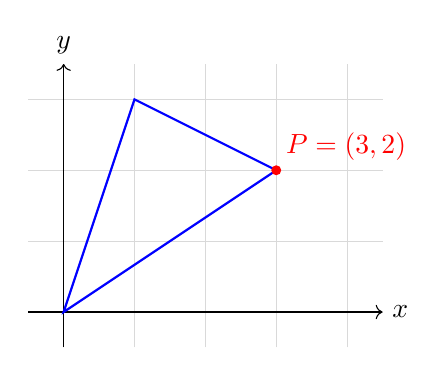
\begin{tikzpicture}[scale=0.9]
  \draw[step=1cm,gray!30,very thin] (-0.5,-0.5) grid (4.5,3.5);
  \draw[->] (-0.5,0) -- (4.5,0) node[right] {$x$};
  \draw[->] (0,-0.5) -- (0,3.5) node[above] {$y$};
  \draw[blue,thick] (0,0) -- (3,2) -- (1,3) -- cycle;
  \fill[red] (3,2) circle (2pt) node[above right] {$P=(3,2)$};
\end{tikzpicture}
\caption{A triangle on a coordinate grid.}
\label{fig:triangle}
\end{figure}

The text following Figure~\ref{fig:triangle} stays below its caption.

\begin{figure}[htbp]
\centering
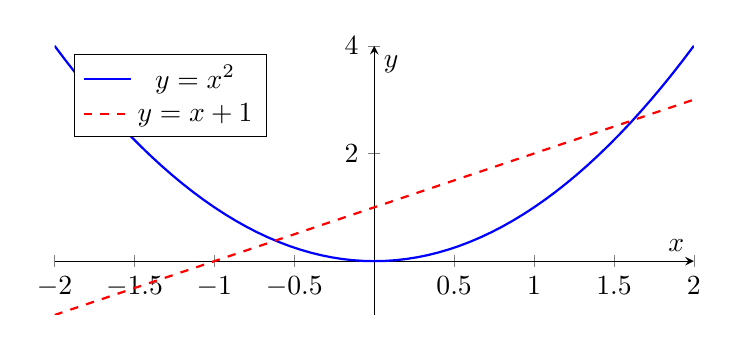
\begin{tikzpicture}
\begin{axis}[width=0.8\linewidth,height=5cm,axis lines=middle,
  xlabel={$x$},ylabel={$y$},domain=-2:2,samples=61,legend pos=north west]
  \addplot[blue,thick] {x^2};
  \addlegendentry{$y=x^2$}
  \addplot[red,dashed,thick] {x+1};
  \addlegendentry{$y=x+1$}
\end{axis}
\end{tikzpicture}
\caption{Two functions drawn with PGFPlots.}
\label{fig:functions}
\end{figure}

\section{Graphs and named nodes}
Named nodes can be joined by edges. This example is a small directed graph;
edit a node coordinate, its label, or the color of an edge in the drawing editor.

\begin{center}
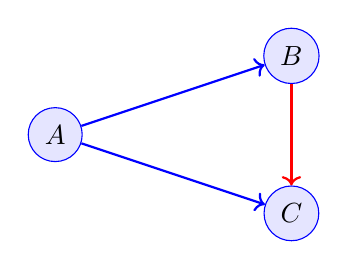
\begin{tikzpicture}
  \node[draw=blue,circle,fill=blue!10] (a) at (0,0) {$A$};
  \node[draw=blue,circle,fill=blue!10] (b) at (3,1) {$B$};
  \node[draw=blue,circle,fill=blue!10] (c) at (3,-1) {$C$};
  \draw[->,blue,thick] (a) -- (b);
  \draw[->,blue,thick] (a) -- (c);
  \draw[->,red,thick] (b) -- (c);
\end{tikzpicture}
\end{center}

\section{Electrical and logic circuits}
TikZ's electrical library places components on \texttt{to} segments. Select a
segment in Plot / data to edit its component options and endpoint. In the
native drawing editor, click a component label to edit its text or formula.

\begin{center}
% Restore these TikZ keys locally; Circuitikz also defines their names.
\begin{tikzpicture}[
  circuit declare symbol=voltage source,circuit declare symbol=resistor,
  circuit declare symbol=capacitor,circuit declare symbol=ground,circuit ee IEC]
  \draw (0,0) to[voltage source={info={$U$}}] (0,3)
    to[resistor={info={$R$}}] (4,3)
    to[capacitor={info={$C$}}] (4,0) -- (0,0);
  \node[ground] at (0,0) {};
\end{tikzpicture}
\end{center}

Named logic-gate terminals keep wires attached to the appropriate input or
output. Changing \texttt{circuit logic US} to \texttt{circuit logic IEC} selects
the rectangular gate symbols.
\begin{center}
\begin{tikzpicture}[circuit logic US]
  \node[and gate,inputs={normal,normal}] (gate) at (0,0) {};
  \node[not gate] (inverse) at (3,0) {};
  \draw (-2,0.7) -- (gate.input 1);
  \draw (-2,-0.7) -- (gate.input 2);
  \draw (gate.output) -- (inverse.input);
  \draw (inverse.output) -- (5,0) node[right] {$\overline{a\land b}$};
\end{tikzpicture}
\end{center}

Circuitikz uses short component names: \texttt{R}, \texttt{C}, \texttt{L} and
\texttt{V}. Qualified label keys avoid a clash with the built-in circuit libraries.
\begin{center}
\begin{circuitikz}[american]
  \draw (0,0) to[V,/tikz/circuitikz/l=$U$] (0,3)
    to[R,/tikz/circuitikz/l=$R$] (3,3) to[L,/tikz/circuitikz/l=$L$] (6,3)
    to[C,/tikz/circuitikz/l=$C$] (6,0) -- (0,0);
\end{circuitikz}
\end{center}

\section{Data and visualization}
PGFPlots accepts coordinate lists and tables as well as functions. The samples
are deliberately small so each data point is easy to change. The first plot
uses semicolon-separated columns and regular tick ranges.

\begin{center}
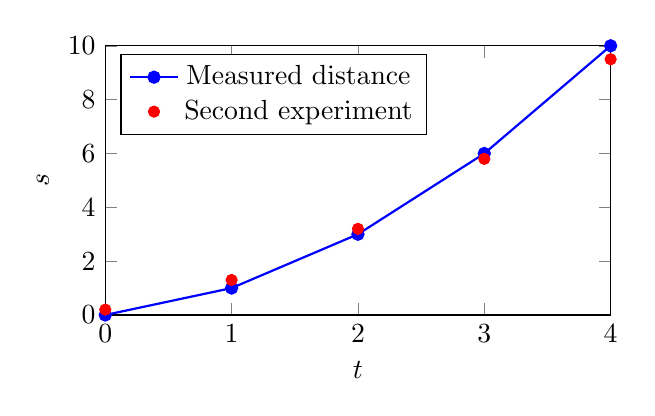
\begin{tikzpicture}
\begin{axis}[width=8cm,height=5cm,xlabel={$t$},ylabel={$s$},
  xmin=0,xmax=4,ymin=0,ymax=10,xtick={0,...,4},ytick={0,2,...,10},
  legend pos=north west]
  \addplot[blue,thick,mark=*] table[col sep=semicolon,x=time,y=distance] {
    time;distance
    0;0
    1;1
    2;3
    3;6
    4;10
  };
  \addlegendentry{Measured distance}
  \addplot[red,only marks] coordinates {(0,0.2) (1,1.3) (2,3.2) (3,5.8) (4,9.5)};
  \addlegendentry{Second experiment}
\end{axis}
\end{tikzpicture}
\end{center}

\begin{center}
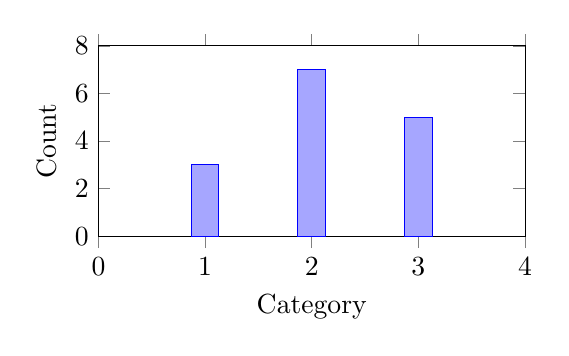
\begin{tikzpicture}
\begin{axis}[width=7cm,height=4cm,ybar,xmin=0,xmax=4,ymin=0,ymax=8,
  xlabel={Category},ylabel={Count}]
  \addplot[draw=blue,fill=blue!35] coordinates {(1,3) (2,7) (3,5)};
\end{axis}
\end{tikzpicture}
\end{center}

TikZ's own data visualization library offers another syntax for a data plot:

\begin{center}
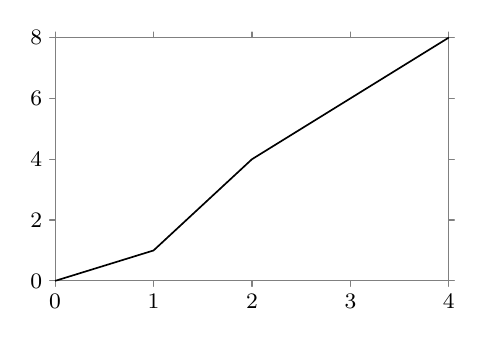
\begin{tikzpicture}
  \datavisualization[scientific axes,visualize as line] data {
    x,y
    0,0
    1,1
    2,4
    3,6
    4,8
  };
\end{tikzpicture}
\end{center}

Named data sets can use different visualizers, colors and legends. The same
axes can include a major grid with three minor grid lines between major steps.
Axis attributes select named columns; included values extend the range.
Click a legend or axis label to edit its text in the native preview.

\begin{center}
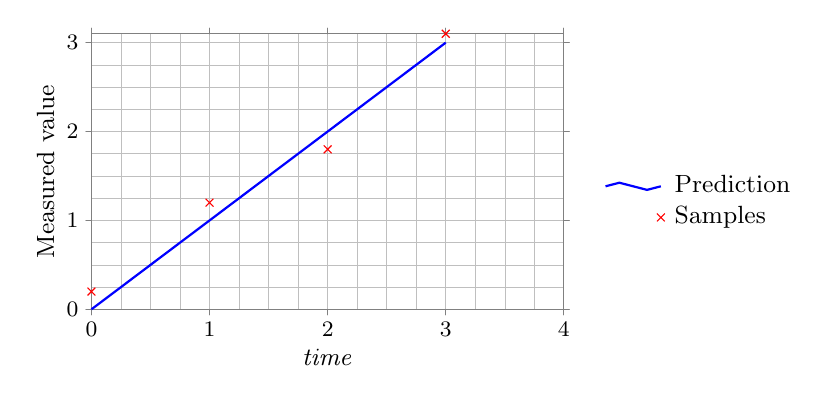
\begin{tikzpicture}
\datavisualization[scientific axes,
  all axes={grid={step=1,minor steps between steps=3}},
  x axis={attribute=time,label,length=6cm,include value={0,4},ticks={step=1}},
  y axis={attribute=value,label={Measured value},length=3.5cm,include value=0,ticks={step=1}},
  visualize as line=prediction,visualize as scatter=experiment,
  prediction={style={visualizer color=blue,thick},label in legend={text={Prediction}}},
  experiment={style={visualizer color=red},label in legend={text={Samples}}}]
data[set=prediction]{
time,value
0,0
1,1
2,2
3,3
}
data[set=experiment]{
time,value
0,0.2
1,1.2
2,1.8
3,3.1
};
\end{tikzpicture}
\end{center}

Function data can share an independent parameter. In the Data set dialog,
edit its variables, functions and options. This example samples a circle:
\begin{center}
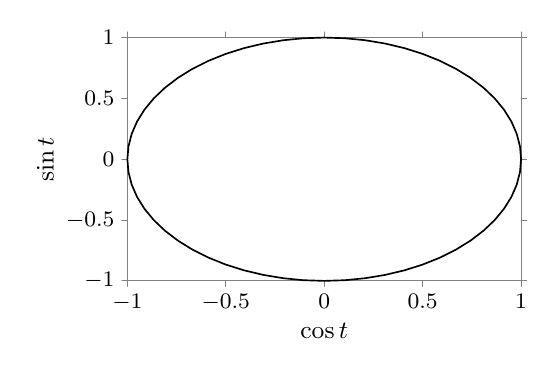
\begin{tikzpicture}
\datavisualization[scientific axes,visualize as line,
  x axis={label={$\cos t$}},y axis={label={$\sin t$}}]
data[format=function]{
var t : interval [0:360] samples 61;
func x = cos(\value t);
func y = sin(\value t);
};
\end{tikzpicture}
\end{center}

Named function data supports scientific notation and braced attribute names:
\begin{center}
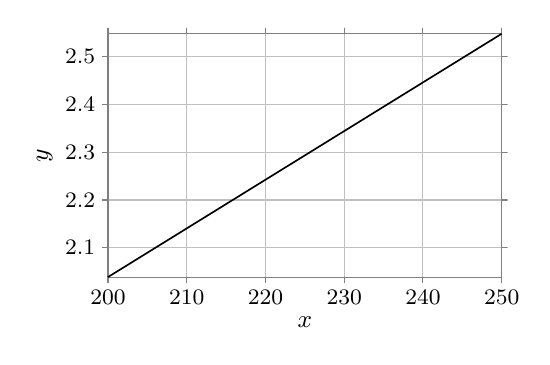
\begin{tikzpicture}
\datavisualization[scientific axes,visualize as line=measured,
  all axes={grid},x axis={label={$x$}},y axis={label={$y$}}]
data[set=measured,format=function]{
var x : interval [200:250];
func y = 1.02e-02*\value{x}+1.00e-05;
};
\end{tikzpicture}
\end{center}

\subsection*{Calculated coordinates and arrow tips}
The calc library supports interpolation, rotation and projection. A let binding
shares calculated coordinates within one path. Arrow tip options stay in braces.
\begin{center}
\begin{tikzpicture}
\coordinate (A) at (0,0);
\coordinate (B) at (4,0);
\draw[gray] (A)--(B);
\draw[blue,-{Kite[open,length=5pt]}] ($(A)!.25!(B)$)--($(A)!.5!90:(B)$);
\draw[red,-{Stealth[length=5pt,width=4pt]}]
  let \p1=(1,2),\n1={sqrt(9)} in (\x1,0)--(\n1,\y1);
\end{tikzpicture}
\end{center}

Polar coordinates set the ray's angle; rotated interpolation constructs a
perpendicular offset. The teal dimension repeats $AP$ above the ray, with dashed
guides connecting the corresponding endpoints. All labels remain editable.
\begin{center}
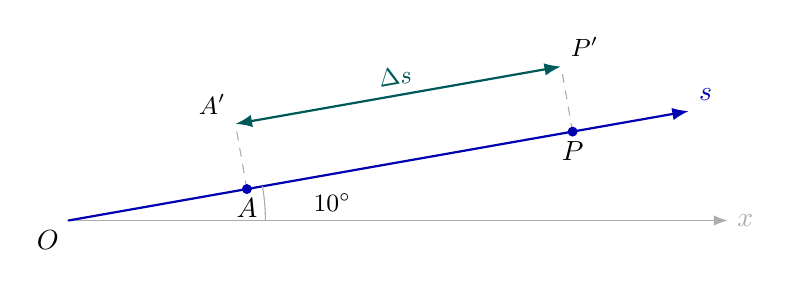
\begin{tikzpicture}[line cap=round,line join=round]
\coordinate[label=below left:$O$] (O) at (0,0);
\coordinate[label=below:$A$] (A) at (10:2.3);
\coordinate[label=below:$P$] (P) at (10:6.5);
\coordinate (Q) at (10:8);
\coordinate[label={[font=\small]above left:$A'$}]
  (Aprime) at ($(A)!.2!90:(P)$);
\coordinate[label={[font=\small]above right:$P'$}]
  (Pprime) at ($(P)+(Aprime)-(A)$);
\draw[gray!65,-{Latex[length=5pt]}]
  (O)--($8.5*cos(10)*(1,0)$) node[right] {$x$};
\draw[blue!70!black,thick,-{Latex[length=6pt]}]
  (O)--(Q) node[above right] {$s$};
\draw[gray!65] (2.5,0) arc [start angle=0,end angle=10,radius=2.5];
\node[font=\small] at (3.35,0.23) {$10^\circ$};
\draw[gray!65,dashed] (A)--(Aprime);
\draw[gray!65,dashed] (P)--(Pprime);
\draw[teal!70!black,thick,arrows={Latex[length=6pt]-Latex[length=6pt]}]
  (Aprime)--(Pprime) node[midway,sloped,above,font=\small] {$\Delta s$};
\fill[blue!70!black] (A) circle (1.8pt);
\fill[blue!70!black] (P) circle (1.8pt);
\end{tikzpicture}
\end{center}

\subsection*{Configurable arrow tips}
Load arrows.meta for named tips and per-tip options. Compare an open Kite,
independent outline/fill colors, and repeated default tips. Arrow options stay
inside braces to keep nested brackets within their option values.
\begin{center}
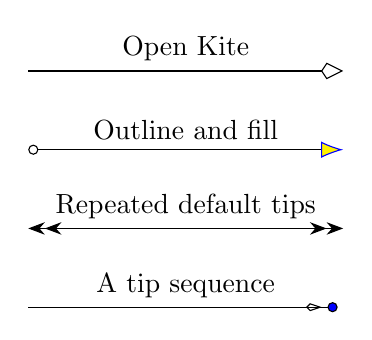
\begin{tikzpicture}
\draw[-{Kite[open,length=8pt,width=6pt]}] (0,0)--(4,0)
  node[midway,above] {Open Kite};
\draw[arrows={Circle[open]-Latex[length=8pt,color=blue,fill=yellow]}]
  (0,-1)--(4,-1) node[midway,above] {Outline and fill};
\draw[>={Stealth[length=6pt]},<<->>] (0,-2)--(4,-2)
  node[midway,above] {Repeated default tips};
\draw[-{[sep=2pt]Kite[open] Circle[fill=blue]}] (0,-3)--(4,-3)
  node[midway,above] {A tip sequence};
\end{tikzpicture}
\end{center}

\section{Trigonometric functions and three dimensions}
PGF uses degrees for trigonometric functions by default. Here the argument of
the sine is converted from radians explicitly.

\begin{center}
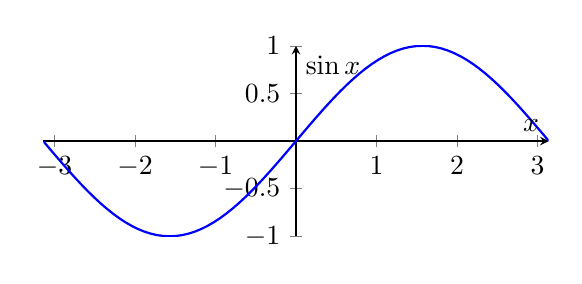
\begin{tikzpicture}
\begin{axis}[width=8cm,height=4cm,domain=-3.14:3.14,samples=81,
  axis lines=middle,xlabel={$x$},ylabel={$\sin x$}]
  \addplot[blue,thick] {sin(deg(x))};
\end{axis}
\end{tikzpicture}
\end{center}

For a surface, choose a modest sample count while editing; increase it for
export if needed. Change the expression or the view angles in the source pane.
The scale beside this surface uses the same viridis palette and a fixed range
from zero to one. Click its ticks or label in the native preview to edit them.

\begin{center}
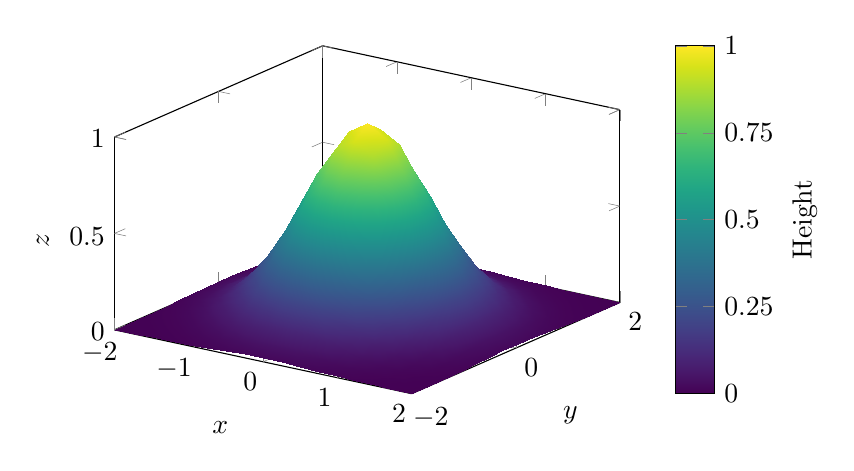
\begin{tikzpicture}
\begin{axis}[width=8cm,height=6cm,view={35}{30},domain=-2:2,
  y domain=-2:2,samples=17,colormap/viridis,xlabel={$x$},ylabel={$y$},zlabel={$z$},
  zmin=0,zmax=1,point meta min=0,point meta max=1,colorbar,
  colorbar style={ylabel={Height},ytick={0,0.25,0.5,0.75,1}}]
  \addplot3[surf,shader=interp,z buffer=sort] {exp(-x^2-y^2)};
\end{axis}
\end{tikzpicture}
\end{center}

The mesh below uses jet and a horizontal color scale. Negative heights are blue,
zero is green, and positive heights are red in both preview backends.

\begin{center}
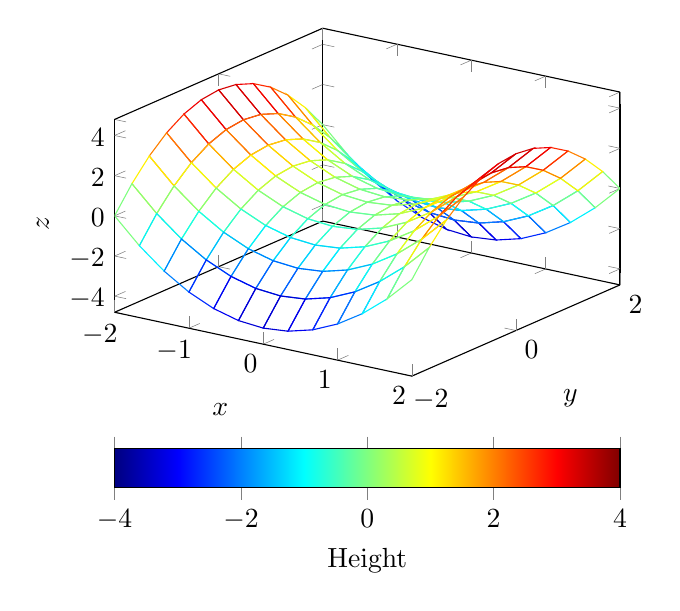
\begin{tikzpicture}
\begin{axis}[width=8cm,height=6cm,view={35}{30},domain=-2:2,
  y domain=-2:2,samples=13,colormap/jet,xlabel={$x$},ylabel={$y$},zlabel={$z$},
  point meta min=-4,point meta max=4,colorbar horizontal,
  colorbar style={xlabel={Height},height=0.5cm,xtick={-4,-2,0,2,4},
    xtick align=outside,axis line style={black,thin}}]
  \addplot3[mesh] {x^2-y^2};
\end{axis}
\end{tikzpicture}
\end{center}

\section{Editing labels and parametric plots}
Use the native preview to click the rotated node or any axis text below.
The path table separates points from inline node labels. In plot settings,
choose parametric coordinates to edit the circle's two expressions.

\begin{center}
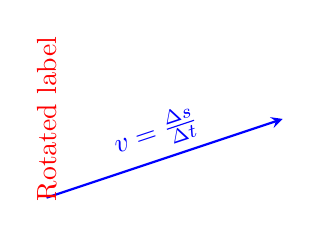
\begin{tikzpicture}
  \draw[blue,thick,->,>=stealth] (0,0) -- (3,1)
    node[midway,sloped,above] {$v=\frac{\Delta s}{\Delta t}$};
  \node[red,rotate=90] at (0,1) {Rotated label};
\end{tikzpicture}
\end{center}

\begin{center}
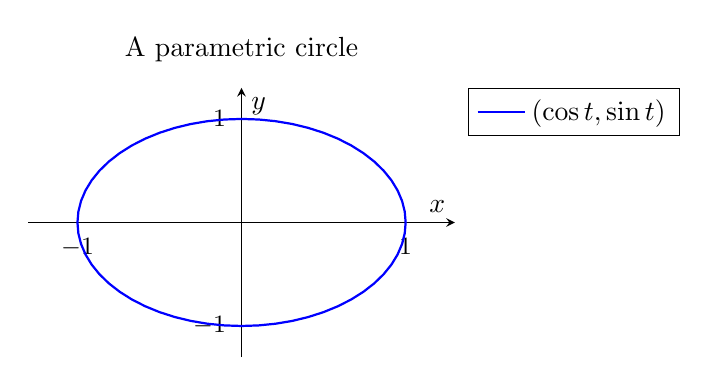
\begin{tikzpicture}
\begin{axis}[width=7cm,height=5cm,axis lines=middle,
  xmin=-1.3,xmax=1.3,ymin=-1.3,ymax=1.3,domain=0:360,samples=61,
  xlabel={$x$},ylabel={$y$},title={A parametric circle},
  xtick={-1,0,1},xticklabels={$-1$,Origin,$1$},
  tick label style={font=\small},legend pos=outer north east]
  \addplot+[blue,mark=none,thick] ({cos(x)},{sin(x)});
  \addlegendentry{$(\cos t,\sin t)$}
\end{axis}
\end{tikzpicture}
\end{center}

The following sections give library examples: positioning, arrows,
decorations, intersections, grouped plots, statistics and filled areas.

The picture code remains ordinary \LaTeX{} source; editing decorations belong to the preview overlay.

\section{Compare drawing backends}
In Settings enable TikZ/PGFPlots instant preview. Cached TeX is the default:
change one coordinate in the triangle and wait for just that diagram to refresh.
The previous cached image remains available while its replacement is generated.
Disable the option to keep an editable gray source box instead.

Choose Native PasTeX for paths, named nodes, math labels, legends, numeric data,
function plots and sampled surfaces or meshes. It is a subset of TikZ/PGFPlots:
arbitrary macros, automatic graph layouts and advanced drawing libraries require
Cached TeX. Unsupported operations remain editable in gray source boxes.
Permanent PDF preview remains the check for complete package output.
Insert, Environment can create an empty figure, table, tikzpicture or axis;
select its package when needed. Edit the outer figure caption and label in place
or through its context menu. Check that following text stays below the caption.

\section{TikZ libraries}
Each example names the libraries it uses. Select Cached TeX in the drawing
editor for complete library output. The source stays editable in either backend.
Library loading belongs in the preamble, through \verb|\usetikzlibrary{...}|
or \verb|\usepgfplotslibrary{...}|.

\subsection{Positioning, shapes, arrows, fit and backgrounds}
Relative positions keep a flowchart together when its text changes. A fitted
background encloses the two processing steps. Try changing a node label,
\texttt{node distance}, or the explicit arrowhead length.
\begin{center}
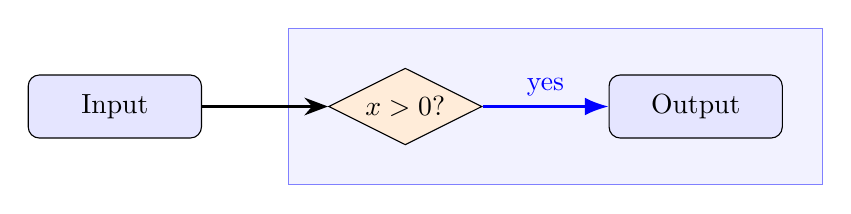
\begin{tikzpicture}[node distance=12mm and 16mm,
  flow step/.style={draw,rounded corners,fill=blue!10,minimum width=22mm,minimum height=8mm},
  decision/.style={diamond,draw,fill=orange!15,aspect=2,inner sep=2pt}]
  \node[flow step] (start) {Input};
  \node[decision,right=of start] (test) {$x>0$?};
  \node[flow step,right=of test] (result) {Output};
  \draw[-{Stealth[length=3mm]},thick] (start) -- (test);
  \draw[-{Latex[length=3mm]},blue,thick] (test) -- node[above] {yes} (result);
  \begin{scope}[on background layer]
    \node[fit=(test)(result),draw=blue!50,fill=blue!5,inner sep=5mm] {};
  \end{scope}
\end{tikzpicture}
\end{center}

\subsection{Calc, intersections, angles and quotes}
The intersection is calculated from two named paths; the midpoint uses the
\texttt{calc} coordinate syntax. The angle label uses the quotes library.
\begin{center}
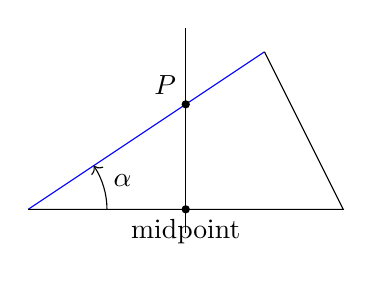
\begin{tikzpicture}
  \coordinate (A) at (0,0); \coordinate (B) at (4,0); \coordinate (C) at (3,2);
  \draw[blue,name path=diagonal] (A) -- (C);
  \draw[name path=vertical] (2,-0.3) -- (2,2.3);
  \path[name intersections={of=diagonal and vertical,by=P}];
  \draw (A) -- (B) -- (C);
  \fill (P) circle (1.5pt) node[above left] {$P$};
  \fill ($(A)!0.5!(B)$) circle (1.5pt) node[below] {midpoint};
  \pic[draw,->,"$\alpha$",angle radius=10mm,angle eccentricity=1.25] {angle=B--A--C};
\end{tikzpicture}
\end{center}

\subsection{Decorations and patterns}
Change the snake amplitude, segment length, or hatch pattern in the options.
\begin{center}
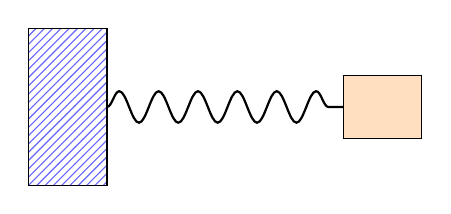
\begin{tikzpicture}
  \fill[pattern=north east lines,pattern color=blue!60] (0,0) rectangle (1,2);
  \draw (0,0) rectangle (1,2);
  \draw[decorate,decoration={snake,amplitude=2mm,segment length=5mm},thick]
    (1,1) -- (4,1);
  \draw[fill=orange!25] (4,0.6) rectangle (5,1.4);
\end{tikzpicture}
\end{center}

\subsection{Graphs}
The graphs library offers a compact syntax for vertices and edges. Automatic
graph-drawing algorithms are a separate library and may require Lua\LaTeX.
\begin{center}
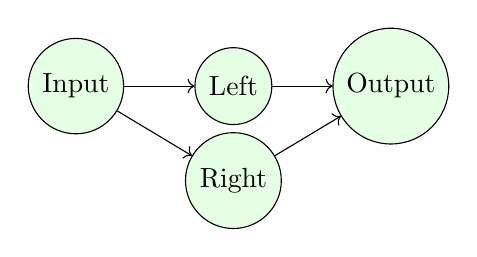
\begin{tikzpicture}[every node/.style={draw,circle,fill=green!10}]
  \graph[grow right=2cm,branch down=12mm] {Input -> {Left,Right} -> Output};
\end{tikzpicture}
\end{center}

\section{PGFPlots libraries}
\subsection{Groupplots}
The two axes share their dimensions and limits. Modify either function, or the
\texttt{group size} and \texttt{horizontal sep} options.
\begin{center}
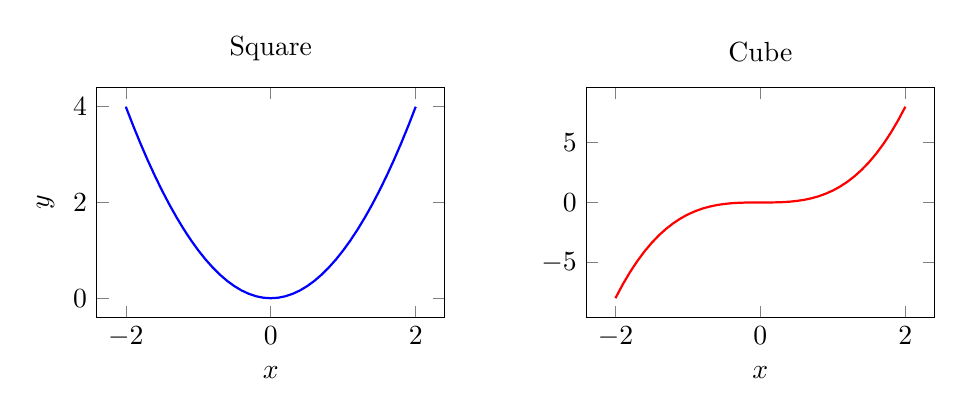
\begin{tikzpicture}
\begin{groupplot}[group style={group size=2 by 1,horizontal sep=18mm},
  width=6cm,height=4.5cm,domain=-2:2,samples=41,xlabel={$x$}]
  \nextgroupplot[title={Square},ylabel={$y$}] \addplot[blue,thick] {x^2};
  \nextgroupplot[title={Cube}] \addplot[red,thick] {x^3};
\end{groupplot}
\end{tikzpicture}
\end{center}

\subsection{Fillbetween}
Named curves define a filled region. Change the expressions or fill opacity.
\begin{center}
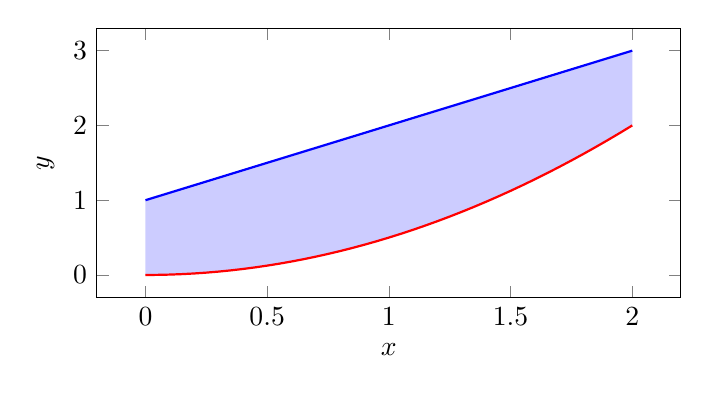
\begin{tikzpicture}
\begin{axis}[width=9cm,height=5cm,domain=0:2,samples=41,xlabel={$x$},ylabel={$y$}]
  \addplot[name path=upper,blue,thick] {x+1};
  \addplot[name path=lower,red,thick] {x^2/2};
  \addplot[blue!20] fill between[of=upper and lower];
\end{axis}
\end{tikzpicture}
\end{center}

\subsection{Statistics}
A prepared box plot declares its quartiles directly; isolated coordinates mark
outliers. Edit the median, quartiles and whiskers to describe another dataset.
\begin{center}
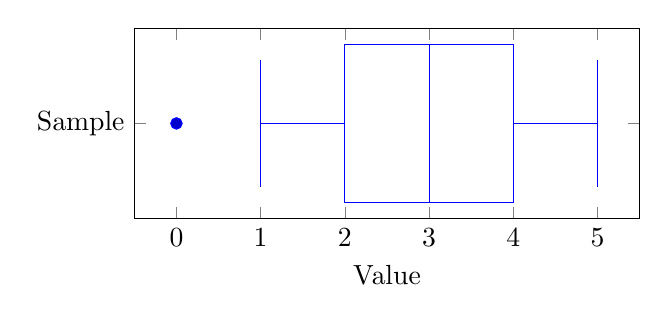
\begin{tikzpicture}
\begin{axis}[width=8cm,height=4cm,ytick={1},yticklabels={Sample},xlabel={Value}]
  \addplot+[boxplot prepared={lower whisker=1,lower quartile=2,median=3,
    upper quartile=4,upper whisker=5}] coordinates {(0,0) (6,0)};
\end{axis}
\end{tikzpicture}
\end{center}

Raw data can use different quantile estimators. The left plot uses PGFPlots'
legacy estimator; the right uses R7 (Excel). Both mark the outlier at 20.
\begin{center}
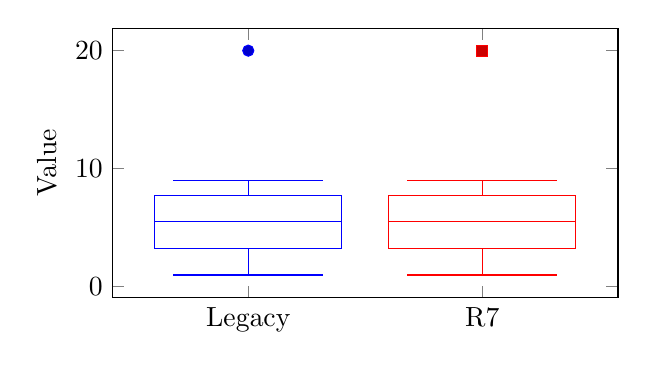
\begin{tikzpicture}
\begin{axis}[width=8cm,height=5cm,boxplot/draw direction=y,
  xtick={1,2},xticklabels={Legacy,R7},ylabel={Value}]
  \addplot+[boxplot] table[row sep=\\,y index=0]
    {data\\1\\2\\3\\4\\5\\6\\7\\8\\9\\20\\};
  \addplot+[boxplot,boxplot/estimator=R7] table[row sep=\\,y index=0]
    {data\\1\\2\\3\\4\\5\\6\\7\\8\\9\\20\\};
\end{axis}
\end{tikzpicture}
\end{center}

\subsection{Polar}
Angles are in degrees. This radial function makes a three-petal curve.
\begin{center}
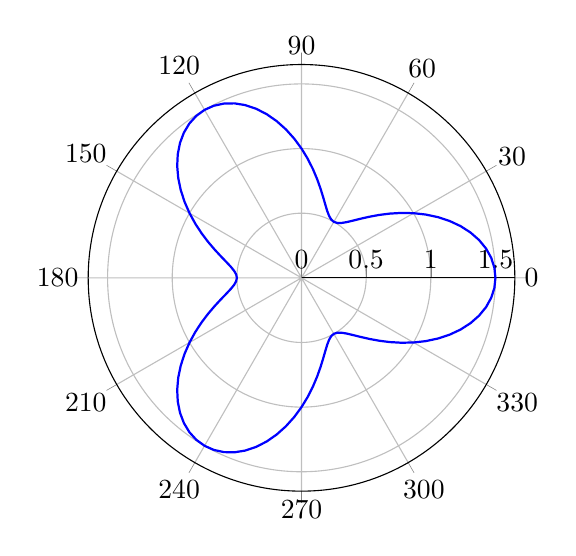
\begin{tikzpicture}
\begin{polaraxis}[width=7cm,height=7cm,domain=0:360,samples=121]
  \addplot[blue,thick] {1+0.5*cos(3*x)};
\end{polaraxis}
\end{tikzpicture}
\end{center}

\subsection{Colormaps and a surface color scale}
The hot palette and its horizontal scale use the same metadata range. The
earlier three-dimensional examples also show viridis and jet.
\begin{center}
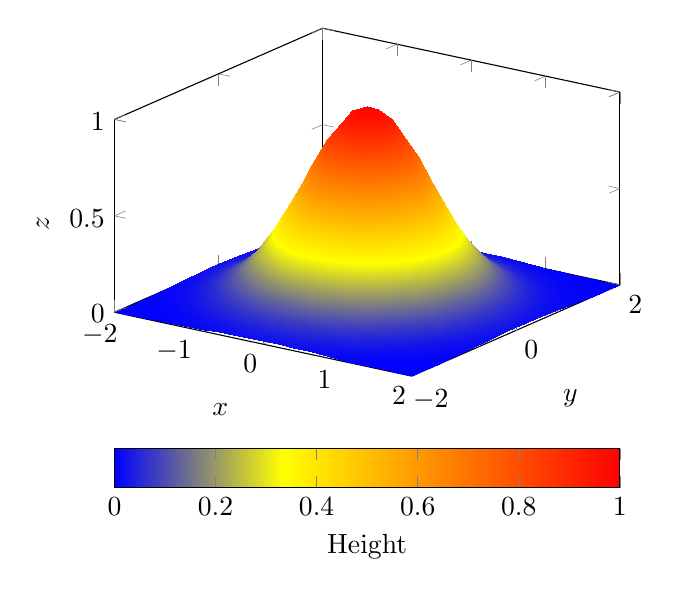
\begin{tikzpicture}
\begin{axis}[width=8cm,height=6cm,view={35}{30},domain=-2:2,y domain=-2:2,
  samples=21,colormap/hot,point meta min=0,point meta max=1,zmin=0,zmax=1,
  colorbar horizontal,colorbar style={xlabel={Height}},xlabel={$x$},ylabel={$y$},zlabel={$z$}]
  \addplot3[surf,shader=interp,z buffer=sort] {exp(-(x*x+y*y))};
\end{axis}
\end{tikzpicture}
\end{center}
\end{document}
